\documentclass[a0,final, portrait]{inriaposter}

\usepackage[utf8]{inputenc}
\usepackage[OT1]{fontenc}
\usepackage[english]{babel}
\usepackage{amsfonts, amsmath, amssymb, amsthm, dsfont, amsthm}
\usepackage{paralist}
\usepackage{wrapfig}

\usepackage{caption}
\usepackage{subcaption} 

\usepackage{graphics}
\usepackage{graphicx}

\providecommand{\mtx}[1]{\mathbf{#1}}

\begin{document}

\sffamily

\postertitle%
{Interactive Task Estimation from \\ \medskip Unlabelled Teaching Signals}
{Jonathan Grizou \; and \; Manuel Lopes \; and \; Pierre-Yves Oudeyer}
{Flowers Team \; ---\; INRIA / ENSTA ParisTech}

\vfill
%\vspace{1cm}
\begin{multicols}{2}
\Large


\blockabstract{
\textbf{Can a robot learn a new task if it does not known how to interpret human instructions?} In the robot social learning literature, robots have access to known sources of information (rewards, correct demonstration, symbolic instructions). Part of the work done in Human Robot Interaction consist of translating human signals (speech, gestures, EEG, etc.) to symbolic meaning usable by the robot. Such signal to meaning mapping requires to train a specific classifier for each user. Training this classifier is time consuming and requires an expert to tune the parameters and collect signal samples. 
\medskip
\par {~~~~~}The idea behind this work is to create calibration free systems that can learn a signal to meaning mapping while learning the task taught by the user. Consider for example the case of a Brain Computer Interaction system that would not require the fastidious calibration procedure.
}

\block{Motivation}
{
\centering
\begin{minipage}{.45\columnwidth}
	\begin{center}
		\includegraphics[width=\columnwidth]{images/scenario.png}
	\end{center}
\end{minipage}
\begin{minipage}{.07\columnwidth}
	\begin{center}

	\end{center}
\end{minipage}
\begin{minipage}{.45\columnwidth}
	\begin{center}
		\includegraphics[width=\columnwidth]{images/problem.png}
	\end{center}
\end{minipage}

\vspace{2cm}
\huge{Can we adpat \textbf{automatically and online} \\ to each user's own preferred teaching signals ? \vspace{2cm}}

\includegraphics[width=\columnwidth, trim=0cm 8cm 0cm 0cm, clip=true]{images/question.png}
}

\block{Problem}
{
\begin{center}
\begin{minipage}{.46\columnwidth}
	\begin{center}
		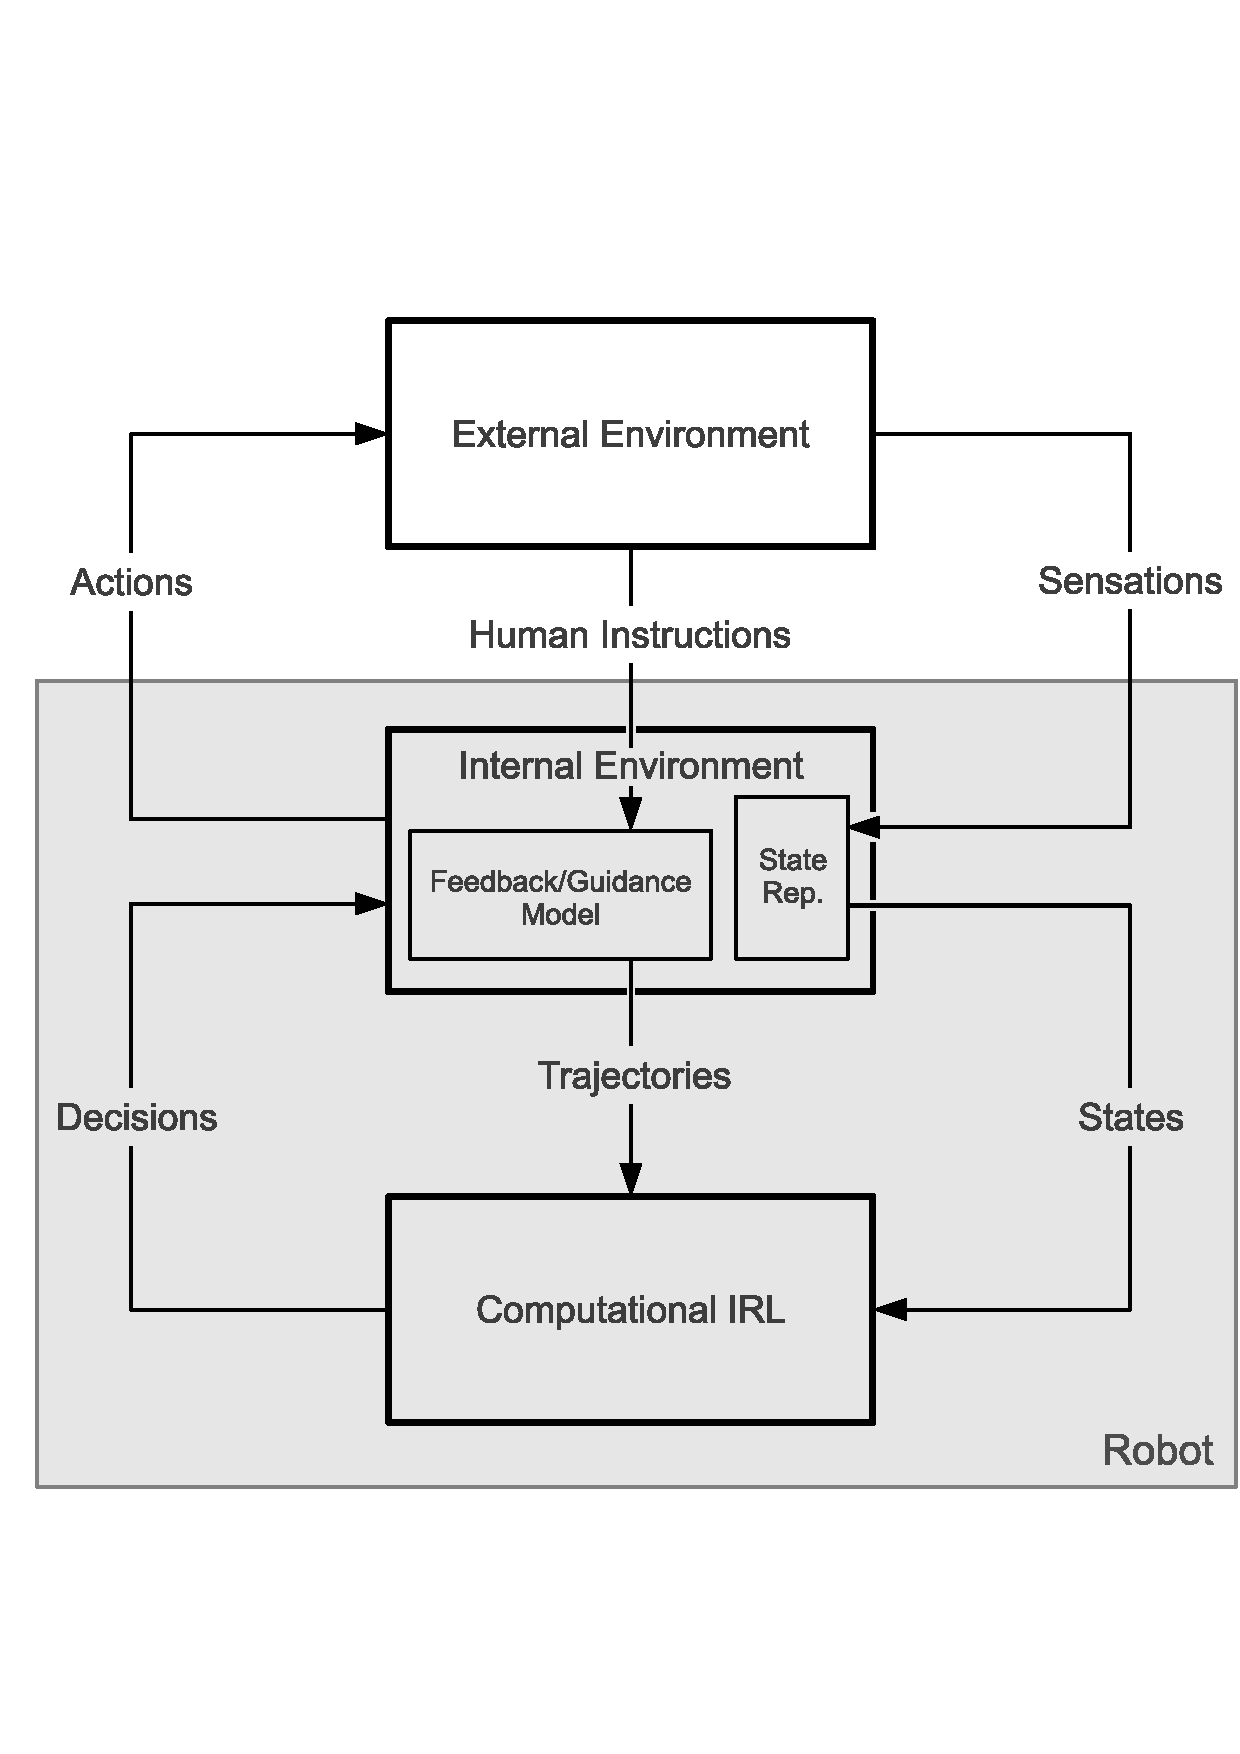
\includegraphics[width=\columnwidth, trim=0cm 0cm 0cm 3cm, clip=true]{images/problem_representation}
	\end{center}
\end{minipage}
\begin{minipage}{.02\columnwidth}
	\begin{center}

	\end{center}
\end{minipage}
\begin{minipage}{.46\columnwidth}
	\begin{center}
		\includegraphics[width=\columnwidth, trim=0cm 0cm 8cm 0cm, clip=true]{images/exemple.png}
	\end{center}
\end{minipage}
\end{center}
\vspace{-2cm}

For successfull communication the human and the robot need to share a common background. Usually it is the meaning of the instructions or demonstrations. In our this work, we rather assume the robot is aware of the set of possible tasks and meanings.
}

\block{Method}
{\begin{center}
\begin{minipage}{.46\columnwidth}
	\begin{center}
		\includegraphics[width=\columnwidth]{images/toy_solution.png}
	\end{center}
\end{minipage}
\begin{minipage}{.02\columnwidth}
	\begin{center}

	\end{center}
\end{minipage}
\begin{minipage}{.442\columnwidth}
	\begin{center}
		\includegraphics[width=\columnwidth]{images/toy_sol.png}
	\end{center}
\end{minipage}
\end{center}
\vspace{1cm}

Our method exploits task constraints, namely optimal policies, to label the feedback signals according to each possible task. For each hypothesis, it is then possible to train a decoder and to compute its expected classification rate. The key point is that these signals are generated from an underlying model that for binary signals has two different classes. Since the right task will assign the right labels to the signals, the expected classification rate is a good measure to identify the user's intended task. 
}

\block{Results}
{
	\begin{center}
		\textbf{1. A HRI Pick and Place Scenario}
		\vspace{0.5cm}
		
		\includegraphics[width=0.3\columnwidth]{images/setup4.png}
		\includegraphics[width=0.3\columnwidth]{images/011}
		\includegraphics[width=0.3\columnwidth]{images/real}

		\vspace{2cm}

		\textbf{2. BCI Control with Human Subjects}
		\begin{minipage}{.49\columnwidth}
		\begin{center}
			With Iñaki Itturrate and\\ Luis Montesano. \vspace{1cm} \\Universidad de Zaragoza, Spain.
		\end{center}
		\end{minipage}
		\begin{minipage}{.49\columnwidth}
		\begin{center}
		\includegraphics[width=0.49\columnwidth, trim=3cm 12cm 33cm 6cm, clip=true]{images/BCI.png}
		\includegraphics[width=0.49\columnwidth, trim=33cm 12cm 3cm 6cm, clip=true]{images/BCI.png}
		\end{center}
		\end{minipage}
		\includegraphics[width=0.49\columnwidth]{images/Avg_evo_likelihood}	
		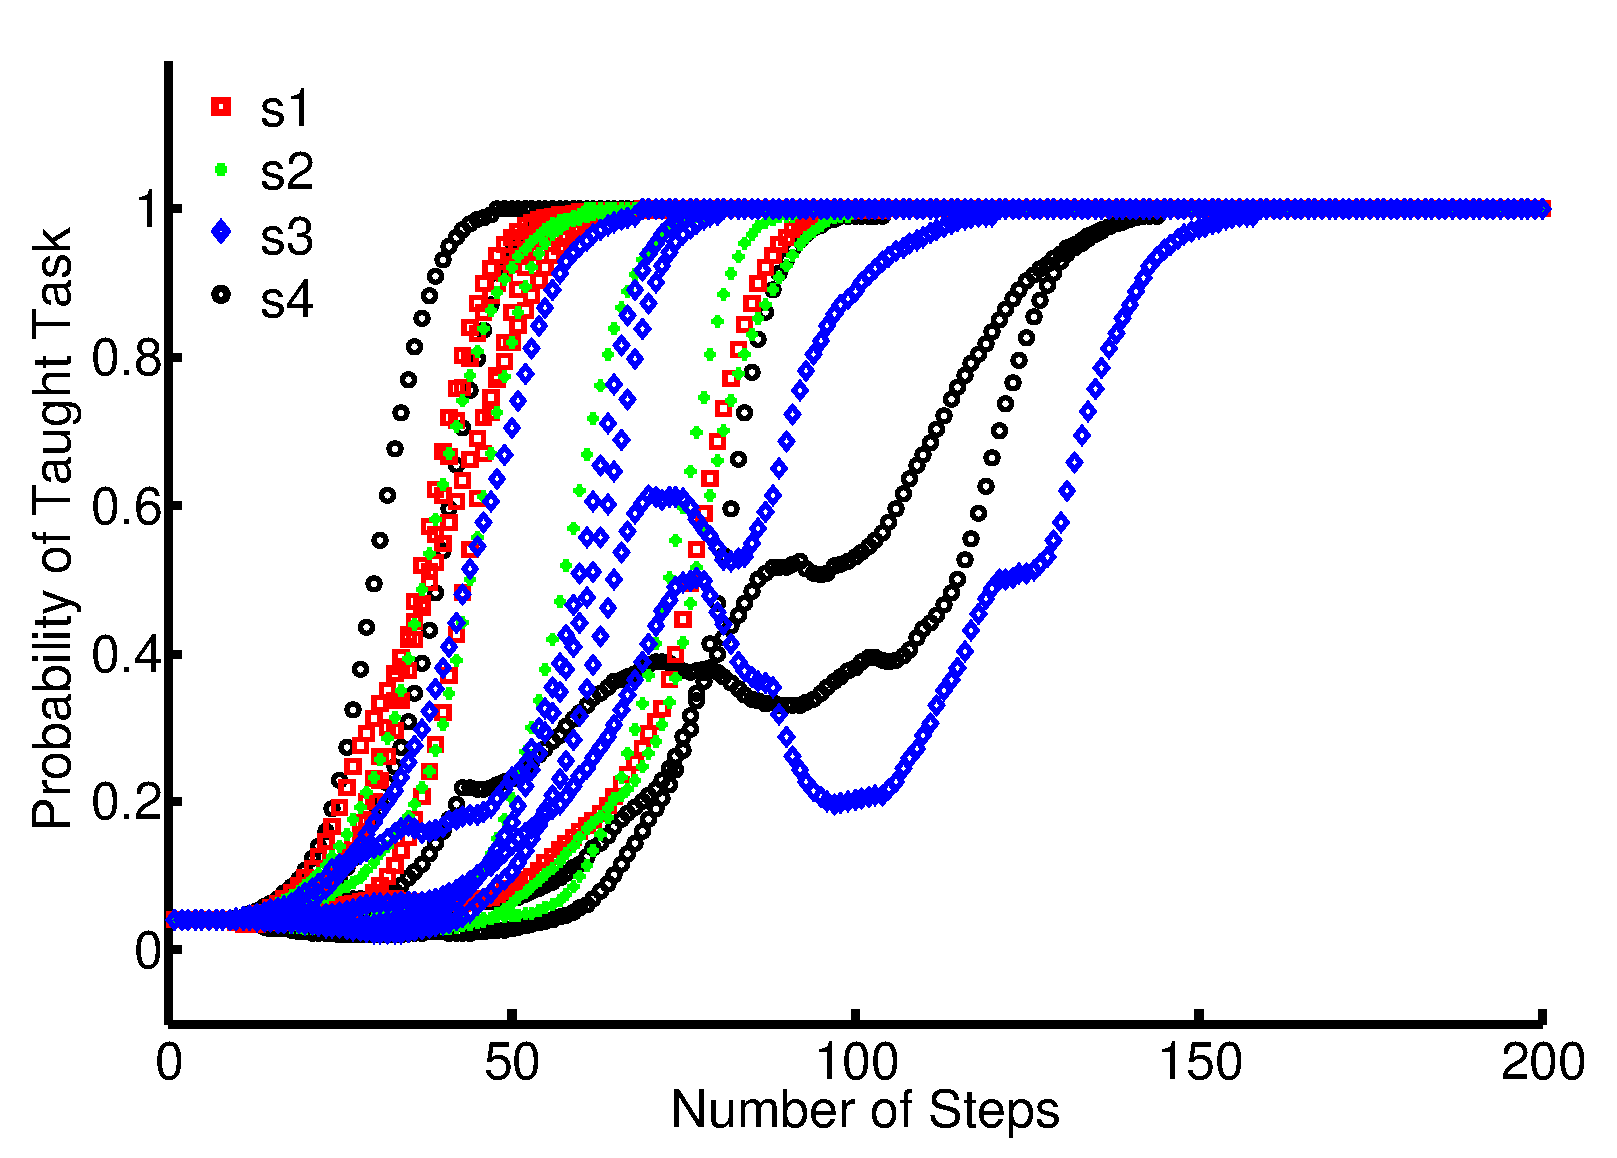
\includegraphics[width=0.49\columnwidth]{images/Evo_likelihood}
	\end{center}				
}


\block{Conclusion}
{
\textbf{Proposed algorithm:}
\begin{inparaenum}
\item Learn a task from unlabeled and noisy instructions.
\item Reuse acquired knowledge.
\end{inparaenum}

\textbf{Of interest:}
\begin{inparaenum}
\item Standard classification technics.
\item Signal expressed as feature vector in RN (can encode facial
expression, gesture, speech, EEG ...).
\end{inparaenum}

\textbf{Limitation:}
\begin{inparaenum}
\item Synchronous and repetitive.
\item Users and robots should share the same meaning model.
\end{inparaenum}
}


\block{Reference}
{
	\vspace{-10pt}
	\bibliographystyle{abbrv}
	\renewcommand{\section}[2]{}% Hack to remove bibliography title
	\bibliography{ref}
	\vspace{-10pt}
}

\end{multicols}
\vfill
\end{document}
